
% -*- coding: utf-8 -*-
% !TEX encoding = UTF-8 Unicode
% !TEX program = xelatex
% !BIB program = biber
% !TEX TS-program = xelatex
% !BIB TS-program = biber
%%
%%
%%
%%
%%
%%
%%  本模板可以使用以下两种方式编译:
%%
%%     1. PDFLaTeX
%%
%%     2. XeLaTeX [推荐]
%%
%%  注意:
%%    1. 在改变编译方式前应先删除 *.toc 和 *.aux 文件,
%%       因为不同编译方式产生的辅助文件格式可能并不相同。
%%
%%
\documentclass[12pt,openright]{book}

\usepackage{ifxetex}
\ifxetex
  \usepackage[bookmarksnumbered]{hyperref}
\else
  \usepackage[unicode,bookmarksnumbered]{hyperref}
\fi

\usepackage[emptydoublepage]{NKThesis}   % 中文
%\usepackage[emptydoublepage,English]{NKThesis} % 英文
\usepackage{amssymb}
%   根据需要选择 biblatex 宏包选项.
\usepackage[backend = biber, defernumbers = true,  sorting=none,  style = gb7714-2015]{biblatex}
\hypersetup{colorlinks=true,
            pdfborder=0 0 1,
            citecolor=black,
            linkcolor=black}
%\usepackage{tikz}
\usepackage{amsmath}

%%%%%%% My Settings %%%%%%%
% \linespread{1.2}
\usepackage{booktabs}
\usepackage{subcaption}
\captionsetup{compatibility=false}
\usepackage{bm}
\renewcommand\bibname{参考文献}
\usepackage{setspace}
\setstretch{1.2}
\graphicspath{{image/}}
\usepackage{algorithm}
\usepackage{algorithmicx}
\usepackage{algpseudocode}
\floatname{algorithm}{算法}
\usepackage{float}
\usepackage{pdfpages}
%%%%%%%%%%%%%%%%%%%%%%%%%%%

\addbibresource{nkthesis.bib}
\DeclareBibliographyCategory{cited}
\AtEveryCitekey{\addtocategory{cited}{\thefield{entrykey}}}

\includeonly{
	./tex/abstract,
	./tex/introduction,
	./tex/relatedwork,
	./tex/method,
	./tex/experiments,
	./tex/summary,
	./tex/references,
	./tex/acknowledgements,
	./tex/appendices,
	./tex/resume
}
\newtheorem{Theorem}{\hskip 2em 定理}[chapter]
\newtheorem{Lemma}[Theorem]{\hskip 2em 引理}
\newtheorem{Corollary}[Theorem]{\hskip 2em 推论}
\newtheorem{Proposition}[Theorem]{\hskip 2em 命题}
\newtheorem{Definition}[Theorem]{\hskip 2em 定义}
\newtheorem{Example}[Theorem]{\hskip 2em 例}
%\newcommand{\upcite}[1]{\textsuperscript{\textsuperscript{\cite{#1}}}}
\begin{document}

%  设置基本信息
%  注意:  逗号`,'是项目分隔符. 如果某一项的值出现逗号, 应放在花括号内, 如 {,}
%
\NKTsetup{%
  论文题目(中文) = 现代绿色化学中的物理有机问题,
  副标题         = ——酵母菌催化反应机理和咪唑类离子液体酸度的研究,
  论文题目(英文) =  Physical Organic Concerns in Green Chemistry: Mechanistic
                   Aspects of Baker's Yeast Mediated Reduction and
                   Measurements of Acidity of Imidazolium Ionic Liquids,
  论文作者       = 张十三,
  学号           = 1020161111,
  指导教师       = 张三\quad 教授,
  申请学位       = 理学硕士,
  培养单位       = 某某学院,
  学科专业       = 某某某某,
  研究方向       = 某某某某,
  中图分类号     = ,
  UDC            = ,
  学校代码       = 10055,
  密级           = 公开,
                   % 公开 | 限制 | 秘密 | 机密, 若为公开, 不填以下三项
  保密期限       = ,
  审批表编号     = ,
  批准日期       = ,
  论文完成时间   = 二〇一九年三月,
  答辩日期       = ,
  论文类别       = 学历硕士,
                   % 博士 | 学历硕士 | 硕士专业学位 | 高校教师 | 同等学力硕士
  学院(单位)       = 某某学院,
  答辩委员会主席       = 李四,
  评阅人       = 李四\quad 王五,
  专业           = 某某某某,
  联系电话       = 1234567,
  Email          = 123@123.com,
  通讯地址(邮编) = 天津市南开区卫津路94号(300071),
  备注           = }

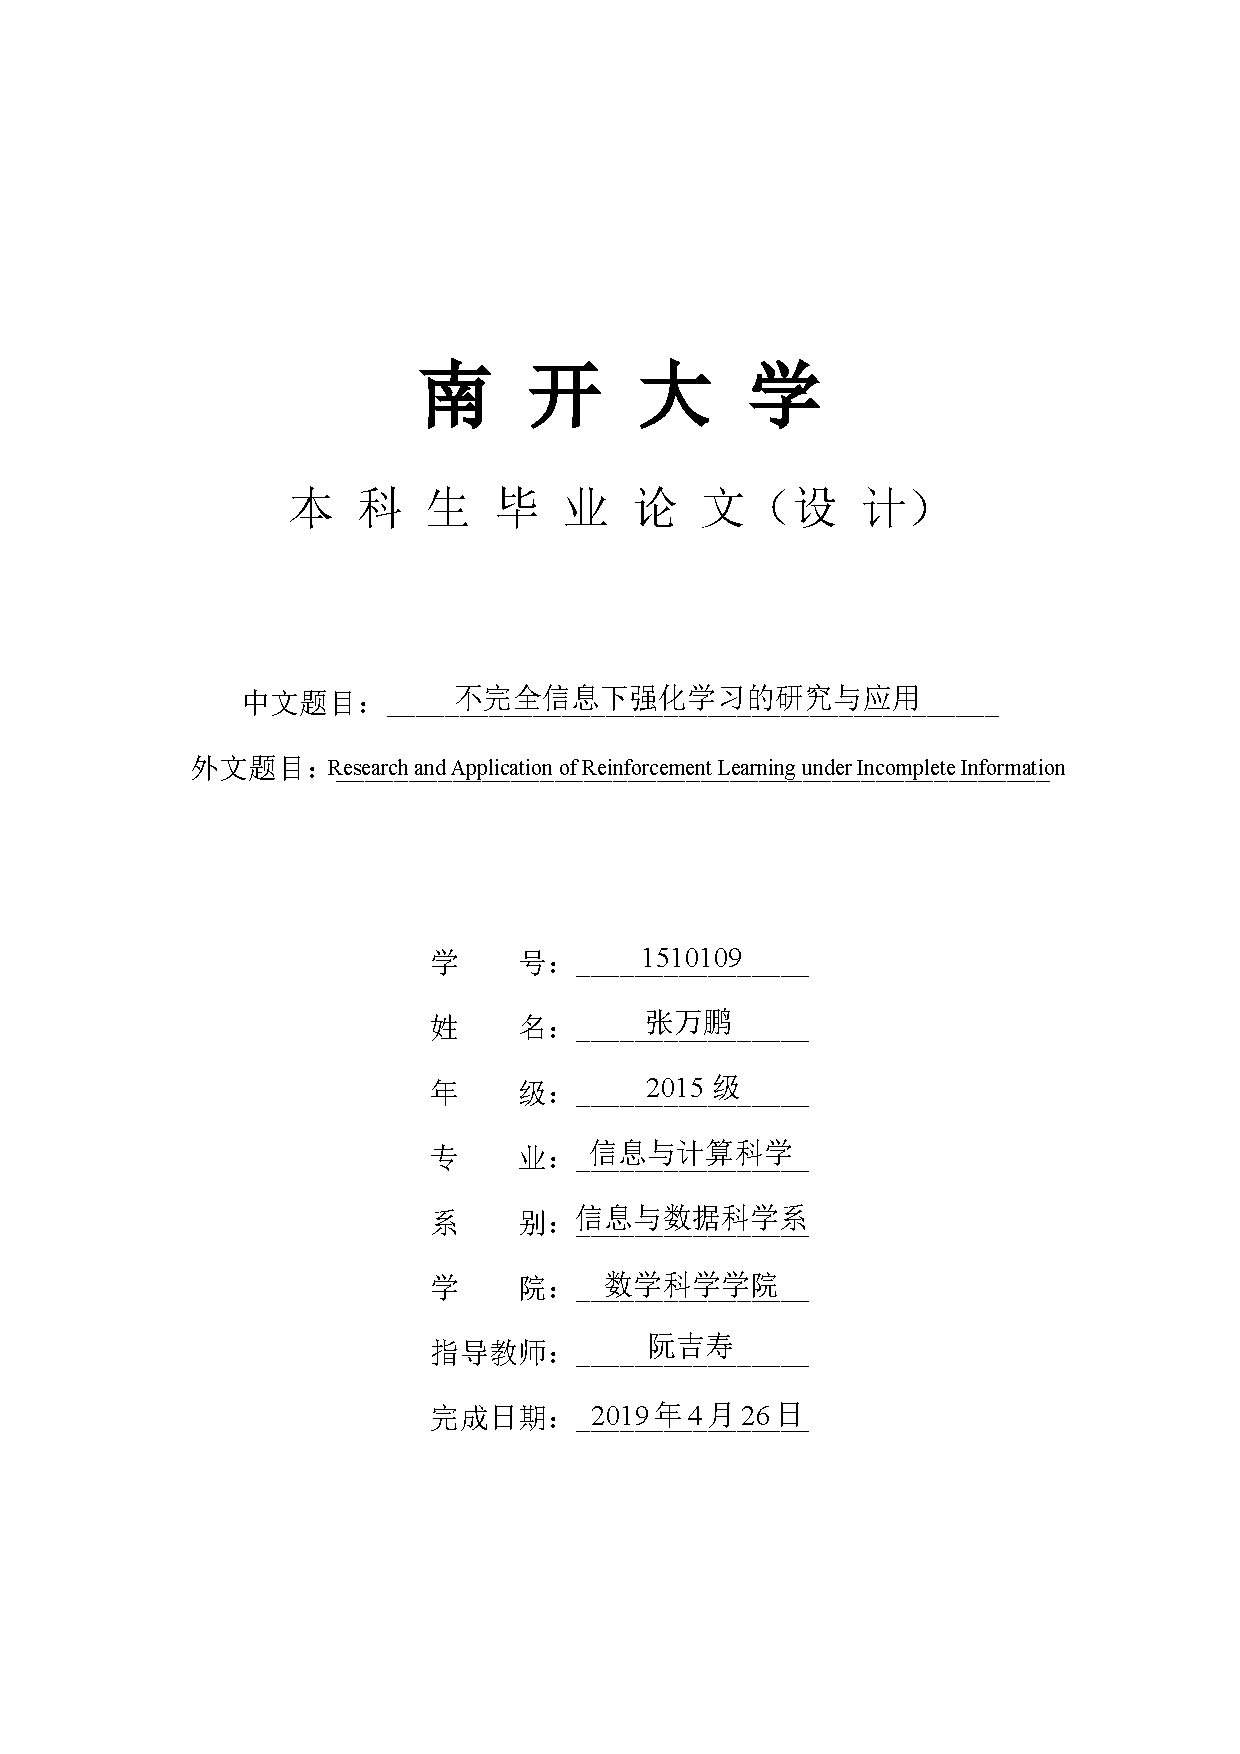
\includepdf[pages={1,2}]{./image/cover.pdf}
% !TeX root = ../main.tex
% -*- coding: utf-8 -*-


\begin{zhaiyao}

传统的强化学习由于理论上的各种假设与限制,只适用于简单的“完全信息博弈问题”,为了能够解决实际中更常见但也更复杂的“不完全信息博弈问题”,本文首先基于模拟采样的思路对传统的理论算法进行改进,解决了不完全信息下难以建模的根本问题。又基于统计学中的 Bootstrap 思想,将模拟采样与 Bootstrap 估计值相结合,改善数据的使用效率,提升模拟近似的准确性。最后再与梯度下降法和深度神经网络相结合,进一步提升算法的运算效率,提出了针对多人不完全信息博弈的“自适应 Deep Q-Learning 算法”。实验表明,“自适应 Deep Q-Learning 算法”能够通过强化学习有效探索出多人博弈技巧,且时间复杂度也表明该算法能够高效快速处理较大数量级的数据集。

\end{zhaiyao}


\begin{guanjianci}
强化学习;不完全信息博弈;模拟采样;神经网络;自适应
\end{guanjianci}



\begin{abstract}


This is the abstract.

\end{abstract}



\begin{keywords}
Thesis; template
\end{keywords}
\tableofcontents
% !TeX root = ../main.tex
% -*- coding: utf-8 -*-
% !TeX root = ../main.tex
% -*- coding: utf-8 -*-

\chapter{绪论}
\label{chpt:introduction}

\section{课题背景}

在传统的机器学习方法中,常见的主要有监督学习和无监督学习\cite{goodfellow2016deep},其中,监督学习是指给定输入 $\boldsymbol{x}$ 和输出 $\boldsymbol{y}$ 的训练集,通过学习输入 $\boldsymbol{x}$ 和输出 $\boldsymbol{y}$ 之间的对应关系的算法;而无监督学习则尝试从不带标签的训练集中推断结论,找到数据之间的隐藏结构\cite{goodfellow2016deep}。

强化学习则是机器学习方法中有别于监督学习和无监督学习的另一类算法,在给定环境下模拟各种行为和动作,接收环境传递的激励和惩罚反馈,自行学习如何行动才能使长期收益最大化。强化学习方法与其他机器学习方法最大的区别,在于强化学习重点关注评价性反馈,而非指导性反馈。其中,评价性反馈是对样本的一个客观评分,而指导性反馈则是明确根据问题背景提供最优解信息\cite{sutton2018reinforcement}。

在传统的强化学习问题中,环境信息会明确给出,如围棋这种双人博弈游戏,由于棋盘盘面有限,且规则简单清晰,对手的当前状态和下一步状态之间的转移概率分布可以得到准确的表示\cite{silver2017mastering}。通过得知这些信息,能够清晰建立准确的环境模型,进而做到通过具体的数学分析来求得最优解。

一场博弈中,如果玩家完美掌握了对手的策略、特征、回报函数等信息,称玩家掌握{\jiacu 完全信息},并称这样的博弈为{\jiacu 完全信息博弈}。前面提到的双人棋类游戏就是完全信息博弈。反之,这样的信息称为{\jiacu 不完全信息},对应的博弈场景称为{\jiacu 不完全信息博弈}或者{\jiacu 动态博弈}\cite{marinatto2000quantum}。

在不完全信息下,由于难以重建环境模型,传统的强化学习算法很难用于处理这类问题\cite{macdermed2011markov}。如在纸牌游戏中,若要建立环境模型,首先需要得到对手可能的手牌概率分布,才能在此基础上建立状态转移概率分布,而不像完全信息下只需建立状态转移概率模型。

不完全信息博弈的这一特点导致其解空间非常大\cite{sandholm2010state},传统的强化学习算法难以克服这一问题,因此需要改进传统的强化学习算法,使得强化学习能够得到更广泛的应用。

\section{论文研究目标和内容}

本文将先介绍传统强化学习的核心思想,然后介绍传统的“基于 Bellman 迭代求解的强化学习算法”,但由于传统强化学习算法只适合处理完全信息博弈问题,因此提出了“基于 Monte Carlo 模拟的强化学习算法”,通过模拟采样来解决不完全信息问题下不能精确建立模型的问题。

进一步地,若只是简单地进行 Monte Carlo 模拟,又将会带来数据效率上的问题,因此基于统计学中的 Bootstrap 思想\cite{efron1994introduction}\cite{2014wzjstatistics}提出了 “Q-Learning 算法”。

最后,为了提升运算上的效率,将 Q-Learning 算法与梯度下降法以及深度神经网络相结合\cite{mnih2013playing},然后针对多模型博弈问题背景做出相应优化,提出了“自适应 Deep Q-Learning 算法”。

为了验证本文所提出的“自适应 Deep Q-Learning 算法”能够有效地处理强化学习问题,选取了一种民间纸牌游戏为仿真实验载体,在其规则下进行仿真模拟实验,运用“自适应 Deep Q-Learning 算法”进行训练学习,来验证这一强化学习算法的学习效果。
% !TeX root = ../main.tex
% -*- coding: utf-8 -*-


\chapter{相关研究综述}
\label{chpt:relatedwork}

\section{强化学习基本框架}

在强化学习中,我们将问题背景划分为“决策者”和“环境”两个部分,其中,“决策者”指算法模型本身,“环境”指决策者以外的信息集合。

环境会随时间发生改变,每个时间下都有特定的“状态”,所有可能出现的状态所组成的集合称为“状态空间”,记作 $\mathcal S$ ,而在时刻 $t$ 对应的状态记作 $S_t\in \mathcal S$ 。

在每个状态下,决策者可以根据环境状态的信息来采取“行动”,将某个状态 $s$ 下所有可采取的行动组成的集合称为“状态 $s$ 下的行动空间”,记作 $\mathcal{A}(s)$ ,特别地,将 $t$ 时刻 $s$ 状态下的特定行动记作 $A_t\in\mathcal{A}(s)$ 。

决策者采取行动 $A_t$ 后,会对环境产生影响,环境则会因此发生改变,由本时刻的状态 $S_t$ 进入下一时刻的状态 $S_{t+1}$ ,同时对决策者当前时刻的行为 $A_t$ 产生一个评价性反馈并传递给决策者,我们将这样的评价性反馈称为“奖励”,记作 $R_{t}\in\mathcal{R}\subset\mathbb{R}$ ,其中 $\mathcal{R}$ 为“奖励空间”,表示所有可能的奖励值组成的集合。

决策者收到环境传来的奖励 $R_{t}$ 后,将能得知环境对刚才的行动 $A_t$ 的客观评价,从而根据该信息来调整自己的“决策策略”,并用于进行下一轮行为决策。而决策的调整,则是强化学习里的重要研究对象。简单而言,调整策略的核心思想是要最大化总收益,即将奖励值的累积求和最大化。

这里引入“回报值”的概念,它是总收益值的一个更规范的描述。定义 $t$ 时刻之后的回报值为 $G_t$ ,其表达式为

\begin{equation}
G_t = R_{t+1}+R_{t+2}+R_{t+3}+\cdots
\end{equation}

特别地,将强化学习问题分为两种类型:片段型和连续型。片段型问题指整体问题能够分解为存在起始状态和终止状态、步骤有限的片段,这些片段均有着相似结构,但不一定完全相同。比如纸牌游戏的一轮牌局就是一个片段,多轮牌局全体构成整体问题。相反,连续型问题则指那些不能分解为子片段的,持续连贯的问题。

在两种问题类型下,回报值 $G_t$ 的公式需做一些调整才能合理。对于片段型问题,从 $t$ 时刻开始,设其所处片段的终止状态对应的时刻为 $T$ ,则应定义

\begin{equation}
G_t = R_{t+1}+R_{t+2}+R_{t+3}+\cdots+R_T
\end{equation}

而对于连续型问题,若简单地将奖励值直接相加,显然会使 $G_t$ 趋于无穷,这将导致无法比较不同行动 $A_t$ 的效果。考虑将 $G_t$ 定义为

\begin{equation}
G_t = R_{t+1}+\gamma R_{t+2}+\gamma^2 R_{t+3}+\cdots = \sum_{k=0}^{\infty}\gamma^kR_{t+k+1}
\end{equation}

其中 $\gamma(0\leq \gamma < 1)$ 为“削减率”,其直观效果是将观测信息的重点集中在较近时刻的奖励值上。

\section{Markov 决策过程}

强化学习的目标是:学习出能由状态信息决定最佳行动的决策策略\cite{sutton2018reinforcement}。状态信息包含了实时信息和一定的历史信息,而显然历史信息不能太过庞大,否则会严重影响学习效率,此时考虑引入 Markov 性质,将问题的模型表示为 Markov 决策过程\cite{howard1960dynamic},这样便能将“历史状态信息”通过状态的转移概率分布体现出来\cite{ross1996stochastic}。

\subsection{Markov 性质}

记全部历史信息的联合概率分布为

\begin{equation}
    \mathrm{Pr}\{S_{t+1}=s',R_{t+1}=r|S_0,A_0,R_1,\ldots,S_{t-1},A_{t-1},R_t,S_t,A_t\}
\end{equation}

记环境的状态转移概率分布为

\begin{equation}
    p(s',r|,s,a) = \mathrm{Pr}\{S_{t+1}=s',R_{t+1}=r|S_t=s,A_t=a\}
\end{equation}

\begin{Definition}
    若有 $p(s',r|s,a) = \mathrm{Pr}\{S_{t+1}=s',R_{t+1}=r|S_0,A_0,R_1,\ldots,S_t,A_t\}$ ,则称这样的问题具有 {\jiacu Markov 性质}。
\end{Definition}

通过引入 Markov 性质,决策者每次进行决策时只需考虑当前状态,因为历史信息也包含在了当前状态之中。

\begin{Definition}
    称一个强化学习问题为 Markov 决策过程,当前仅当这个强化学习问题满足 Markov 性质\cite{sutton2018reinforcement}\cite{howard1960dynamic}。
\end{Definition}

根据之前的定义,$p(s',r|s,a) =\mathrm{Pr}\left\{S_t=s',R_t=r|S_{t-1}=s,A_{t-1}=a\right\}$ ,且有 $\sum_{s'\in\mathcal{S}}\sum_{r\in\mathcal{R}}p(s',r|s,a)=1$ 。

其中,$p(s',r|s,a)$ 表示决策者在处于状态 $s$ 时做出行动 $a$ 的条件下,进入下一个状态 $s'$ 并收到奖励值反馈 $r$ 的概率分布。

\subsection{状态价值函数与行为价值函数}

强化学习的核心是通过对行动的评价来调整决策策略,我们需要将行动的评价以及决策策略都定义为函数,才能进行进一步的具体分析。

记概率空间为 $\mathcal P$ ,将策略函数定义为映射:$\pi:\mathcal{S}\times\mathcal{A}\to \mathcal{P}$ 。特别地,条件概率 $\pi(a|s)$ 表示决策者在状态 $s$ 时选择行动 $a$ 的概率分布。

确定了策略 $\pi$ 后,我们定义状态值函数:

\begin{equation}
    v_{\pi}(s) =\mathbb{E}_{\pi}\left[G_t|S_t=s\right]=\mathbb{E}_{\pi}\left[\sum_{k=0}^{\infty}\gamma^kR_{t+k+1}\mid S_t=s\right], \forall s \in \mathcal{S}
\end{equation}

以及行动值函数:

\begin{equation}
    q_{\pi}(s,a) =\mathbb{E}_{\pi}\left[G_t|S_t=s,A_t=a\right]=\mathbb{E}_{\pi}\left[\sum_{k=0}^{\infty}\gamma^kR_{t+k+1}\mid S_t=s,A_t=a\right]
\end{equation}

$v_\pi(s)$ 表示从状态 $s$ 开始,决策者之后若完全遵守策略 $\pi$ 来采取行动,所能得到的期望回报值。而 $q_\pi(s,a)$ 表示在状态 $s$ 下,已经采取了某个行动 $a$ ,之后若完全遵守策略 $\pi$ 采取行动,所能得到的期望回报值。

\section{基于 Bellman 最优方程的强化学习算法}

\subsection{Bellman 最优方程}

\begin{Theorem}
    在有限马尔可夫决策过程中,当前状态 $s$ 与未来所有可能状态 $s'$ 满足 Bellman 方程关系,即
    \begin{equation}
        v_{\pi}(s) = \sum_a\pi(a|s)\sum_{s',r}p(s',r|s,a)\left[r+\gamma v_\pi(s') \right]
    \end{equation}
\end{Theorem}

\begin{proof}
    由定义,显然有

    \[
    \begin{aligned} v_\pi(s) & = \mathbb{E}_\pi[G_t\,|\,S_t=s] \\ &=\mathbb{E}_\pi \left[\sum_{k=0}^\infty\gamma^kR_{t+k+1}\,|\,S_t=s \right] \\ &= \mathbb{E}_\pi \left [R_{t+1}+\gamma\sum_{k=0}^\infty\gamma^kR_{t+k+2}\,|\,S_t=s \right] \\ &=\sum_a\pi(a|s)\sum_{s'}\sum_rp(s',r|s,a)\left[r+\gamma \mathbb{E}_\pi \left[\sum_{k=0}^\infty\gamma^kR_{t+k+2}\,|\,S_{t+1}=s' \right] \right] \\ &= \sum_a\pi(a|s)\sum_{s',r}p(s',r|s,a)\left[r+\gamma v_\pi(s') \right], \qquad \forall s \in \mathcal S \end{aligned}
    \]

    得证。
\end{proof}

强化学习问题的目标是找到解决问题的最优策略,这一目标的前提是得到最优策略对应的价值函数,才能根据这个价值函数推出最优策略。

\begin{Definition}
    在策略空间 $\mathcal{P}$ 中存在且至少存在一个策略优于其他所有策略,称满足这一条件的策略为\textbf{最优策略},其对应的价值函数 $v_*(s)$ 和 $q_*(s,a)$ 分别称为{最优状态值函数}、\textbf{最优行动值函数}。
\end{Definition}

在该定义的基础上,可以得到 Bellman 最优方程\cite{howard1960dynamic}。

\begin{Theorem}
    $v_*$ 作为价值函数时,状态 $s$ 与未来所有可能状态 $s'$ 满足 Bellman 最优方程关系,即
    \begin{equation}
        v_*(s)=\max_{a}\sum_{s',r}p(s',r \mid s,a)[r+\gamma v_*(s')]
    \end{equation}
\end{Theorem}

\begin{proof}
    在最优策略下,显然有

     \[
    \begin{aligned}v_*(s) &= \max_{a\in \mathcal A(s)}q_{\pi_*}(s,a) \\ &=\max_a \mathbb{E}_{\pi_*} \left[G_t \mid S_t=s, A_t=a \right] \\ &= \max_a \mathbb{E}_{\pi_*} \left[\sum_{k=0}^\infty \gamma^kR_{t+k+1} \mid S_t=s,A_t=a \right] \\ &= \max_a \mathbb{E}_{\pi_*} \left[R_{t+1}+\gamma \sum_{k=0}^\infty\gamma^kR_{t+k+2}\mid S_t=s,A_t=a \right] \\ &= \max_a \mathbb{E}[R_{t+1}+\gamma v_*(S_{t+1}) \mid S_t=s,A_t=a] \\ &=\max_{a}\sum_{s',r}p(s',r \mid s,a)[r+\gamma v_*(s')]\end{aligned}
    \]

    得证。
\end{proof}

Bellman 最优方程的行动价值函数形式为

\begin{equation}
    q_*(s,a) = \sum_{s',r}p(s',r \mid s,a)\left[r+\gamma \max_{a'}q_*(s',a') \right]
\end{equation}

\begin{Definition}
    显然在行动空间 $\mathcal{A}(\mathcal{S})$ 中存在且至少存在一个行动,其行动价值函数值能取到 $v_*$,记该行动为 $a_*$,如果一个策略只将非零概率分配给这些行动,称这个策略是最优策略。
\end{Definition}

至此,已经得到一个最基本的强化学习算法:求解 Bellman 最优方程得到最优价值函数 $v_*$ 和 $q_*$ ,根据最优价值函数确定出最优策略。但由于 Bellman 方程较为复杂,直接求解计算难度较大,所以在实际中并不实用,需要对其进行一定的改进。

\subsection{迭代法近似求解 Bellman 方程}

为了提升求解 Bellman 方程的效率,考虑采用 Jocobi 迭代法\cite{2007numanalysis}。Jacobi 迭代法的收敛条件为

\begin{Theorem}\label{the:jacobi}
    对于方程组 $\boldsymbol{x}_{k+1} = \boldsymbol{Cx}_{k}+\boldsymbol{b}$ ,给定方程组的一个初始近似解 $\boldsymbol{x}_0$ ,由前式迭代产生的序列 $\left\{\boldsymbol{x}_0,\boldsymbol{x}_1,\boldsymbol{x}_2,\cdots,\boldsymbol{x}_k,\cdots\right\}$ 收敛的充分必要条件是矩阵 $\boldsymbol{C}$ 满足条件 $\lim\limits_{k \rightarrow \infty} \boldsymbol{C}^{k}=\boldsymbol{O}$ 。
\end{Theorem}

\begin{Theorem}\label{the:bellmanjacobi}
    Bellman 方程可由 Jacobi 迭代法求得收敛解。
\end{Theorem}

\begin{proof}

将 Bellman 方程的迭代形式为

\begin{equation}\label{eq:itebellman}
    v_{k+1}(s) = \sum_a\pi(a\mid s)\sum_{s',r}p(s',r \mid s,a)[r+\gamma v_k(s')]
\end{equation}

设状态空间 $\mathcal S$ 中有 $n$ 个不同的状态,则可将该 Bellman 迭代式具体展开为

\begin{equation}
    \begin{aligned}
        v_{k+1}(s_1)=&c_{11}v_k(s_1)+c_{12}v_k(s_2)+\cdots+c_{1n}v_k(s_n)+b_1\\
        v_{k+1}(s_2)= & c_{21}v_k(s_1)+c_{22}v_k(s_2)+\cdots+c_{2n}v_k(s_n)+b_2\\
        &\vdots\\
        v_{k+1}(s_n)= & c_{n1}v_k(s_1)+c_{n2}v_k(s_2)+\cdots+c_{nn}v_k(s_n)+b_n\\
        \end{aligned}
\end{equation}

其中

\begin{equation}
    \begin{aligned}
        c_{ij} &=\sum_a\pi(a\mid s_i)\sum_{r}p(s_j,r \mid s_i,a)\gamma\\
        &\leq \sum_a\pi(a\mid s_i)\sum_{s_j,r}p(s_j,r \mid s_i,a)\gamma=\gamma
    \end{aligned}
\end{equation}

\begin{equation}
    b_{i} =\sum_a\pi(a\mid s_i)\sum_{r}p(r\mid s_i,a)r
\end{equation}

记

\begin{equation}
    \boldsymbol{C} =
    \left(\begin{array}{cccc}
    c_{11} & c_{12} & \cdots & c_{1n} \\
    c_{21} & c_{22} & \cdots & c_{2n} \\
    \vdots & \vdots & \ddots & \vdots \\
    c_{n1} & c_{n2} & \cdots & c_{nn}
    \end{array}\right)
\end{equation}

则可简记 Bellman 迭代式的矩阵形式为

\begin{equation}\label{eq:bellmaneq}
    \boldsymbol{v}_{k+1} =\boldsymbol{Cv}_k+\boldsymbol{b}
\end{equation}

对于 Bellman 迭代式 \ref{eq:bellmaneq} ,由于 $0\leq\gamma<1$ ,显然有

\begin{equation}
    \lim_{k\rightarrow \infty} \boldsymbol{C}^k = \lim_{k\rightarrow \infty}\left(\begin{array}{cccc}
    \gamma & \gamma & \cdots & \gamma \\
    \gamma & \gamma & \cdots & \gamma \\
    \vdots & \vdots & \ddots & \vdots \\
    \gamma & \gamma & \cdots & \gamma
    \end{array}\right)^k = \boldsymbol{O}
\end{equation}

因此由定理 \ref{the:jacobi} 可知,Bellman 迭代式 \ref{eq:itebellman} 可由 Jacobi 迭代法快速求解,并且解收敛,定理得证。

\end{proof}

根据定理\ref{the:bellmanjacobi}的结论,对于任意强化学习问题,都可以给出一个基于 Bellman 迭代求解的强化学习算法:

\begin{algorithm}[H]
    \caption{基于 Bellman 迭代求解的强化学习算法}
    \begin{algorithmic}[1] %每行显示行号
        \State 初始化向量 $V(s), \forall s\in \mathcal S$
        \Repeat
        \State $\Delta\leftarrow 0$
        \For{每个 $s\in\mathcal S$}
        \State $v\leftarrow V(s)$
        \State $V(s)\leftarrow \max_a\sum_{s',r}p(s',r|s,a)[r+\gamma V(s')]$
        \State $\Delta \leftarrow \max(\Delta,|v-V(s)|)$
        \EndFor
        \Until{ $\Delta<\theta$}
        \State
        \State $\pi(s)=\arg\max_a\sum_{s',r}p(s',r|s,a)[r+\gamma V(s')]$
        \State 输出策略 $\pi$
    \end{algorithmic}
\end{algorithm}
% !TeX root = ../main.tex
% -*- coding: utf-8 -*-
% !TeX root = ../main.tex
% -*- coding: utf-8 -*-

\chapter{基于模拟采样的强化学习算法}

基于 Markov 性质的前提,即在 Markov 决策过程中,之前给出的基于迭代求解 Bellman 方程的强化学习算法非常简洁清晰,但该算法对环境条件的依赖性较强,并且还需要显示地确定环境的动态分布 $p(s',r|s,a)$ ,这正是阻碍不完全信息博弈问题直接采用传统强化学习方法的最大难题。

在传统的“完全信息博弈”中,如围棋这类双人博弈问题,由于棋盘盘面有限,且规则简单清晰,对手的当前状态和下一步状态之间的转移概率分布可以得到准确的表示\cite{silver2017mastering},因此可以很方便地确定环境的动态分布 $p(s',r|s,a)$,但对于实际中更常见且更复杂的“不完全信息博弈”,如纸牌类游戏,若要建立环境模型,首先需要得到对手可能的手牌概率分布,才能在此基础上建立状态转移概率分布,然而对手的手牌概率分布是随着游戏进行而动态变化的,显然并不能准确得知 $p(s',r|s,a)$ ,传统的强化学习算法很难克服这一问题\cite{sutton2018reinforcement},所以需要在其基础上做进一步改进,通过模拟采样的方法来获取和近似估计回报值,避免对环境进行模型重建。

\section{Monte Carlo 模拟}

Monte Carlo 方法\cite{goodfellow2016deep}\cite{robert2013monte}也称统计模拟方法,上一章的基于解 Bellman 方程的强化学习算法,由于依赖环境动态信息 $p(s',r|s,a)$ ,在不完全信息下无法得到此式,仅适合处理传统的完全信息问题,但借由 Monte Carlo 模拟方法,可以通过模拟和采样来近似地获得环境信息,进而也能使用强化学习来解决不完全信息问题。

在未知 $p(s',r|a,s)$ 的情况下,算法不能使用的根本原因在于无法计算 Bellman 方程 \ref{eq:bellmaneq} 中的 $\sum_{s',r}p(s',r|s,a)[r+\gamma v(s')]$ ,即无法清晰地预知未来的状态与反馈信息,关键原因在于每一步的奖励值 $r$ 无法取得,而如果采用 Monte Carlo 方法进行模拟,可以进行大量模拟实验,通过计算样本回报值的均值,便能有效解决这一点。

记某个回合中通过模拟得到的反馈数据序列为 $\left\{R_0, R_1, R_2, \ldots, R_T\right\}$ ,在这一回合中,可计算出时刻 $t$ 对应的回报值

\begin{equation}
    G_t = R_{t+1} + \gamma R_{t+2} + \gamma^2 R_{t+3} + \cdots + \gamma^{T-t-1} R_T
\end{equation}

计算 Monte Carlo 模拟获得的回报值均值,可以作为价值函数的估计,即可得到基于 Monte Carlo 模拟的强化学习算法:

\begin{algorithm}[H]
    \caption{基于 Monte Carlo 模拟的强化学习算法}
    \begin{algorithmic}[1] %每行显示行号
        \State 将 $\pi$ 初始化为一个随机策略
        \State 初始化向量 $Q(s,a), \forall s\in \mathcal S,a\in \mathcal{A}(s)$
        \State 将 $Returns(s,a)$ 初始化为一个空数组,$\forall s\in\mathcal S,a\in\mathcal{A}(s)$
        \Loop
        \State 随机选取初始状态 $S_0\in\mathcal S$ 和初始行动 $A_0\in\mathcal{A}(S_0)$
        \State 服从现有策略 $\pi$ 与环境交互生成一个回合片段
        \State 得到 $S_{0}, A_{0}, R_{1}, S_{1}, A_{1}, R_{2}, \ldots, S_{T-1}, A_{T-1}, R_{T}$
        \State $G\leftarrow 0$
        \For{回合中的每一步 $t=T-1, T-2, \ldots, 0$, }
        \State $G \leftarrow \gamma G+R_{t+1}$
        \If{$S_t,A_t$ 在 $S_{0}, A_{0}, S_{1}, A_{1} \ldots, S_{t-1}, A_{t-1}$ 中出现过}
        \State 将 $G$ 追加进数组 $Returns(S_t,A_t)$
        \State $Q(S_t,A_t)\leftarrow \mathrm{average}(Returns(S_t,A_t))$
        \State $\pi(S_t)\leftarrow \arg\max_aQ(S_t,a)$
        \State 跳出本层循环
        \EndIf
        \EndFor
        \EndLoop
        \State
        \State 输出最终策略 $\pi$
    \end{algorithmic}
\end{algorithm}

\section{Bootstrap 自助学习}

Monte Carlo 算法的价值函数更新式为

\begin{equation}\label{eq:mcupdate}
    V(S_t)\leftarrow V(S_t)+\alpha\left[G_t-V(S_t)\right]
\end{equation}

在 Monte Carlo 算法中,由于需要等待一个完整的片段结束,得到每个时间点的奖励值 $R_t$,才能返回到之前各时间点求得对应的回报值 $G_t = R_{t+1}+\gamma R_{t+2}+\gamma^2 R_{t+3}+\cdots+\gamma^{T-t-1} R_T$ 。这一缺点限制了算法的使用场景,其高延迟使得算法无法处理实时学习问题,而 Monte Carlo 本身需要等待一个完整回合结束的特点也导致无法处理连续型问题。

为了能够做到实时更新,即需要在每个时间点 $t$ 得到当前反馈奖励值 $R_t$ 时能够即使更新,而非累积足够多反馈奖励值才去更新,故考虑结合统计学中的 Bootstrap 思想\cite{efron1994introduction}\cite{2014wzjstatistics},利用“重抽样”的思想来尽可能利用信息价值,根据当前时刻 $t$ 下的信息进行一定程度的“再利用”,使用估计值来替换 $G_t$ 。

具体地,记 $\widehat{V}(S_{t})$ 表示 $V({S_t})$ 的一个估计值,则有

\begin{equation}\label{eq:vhat}
    \widehat{V}(S_{t+1}) \approx R_{t+2} + \gamma R_{t+3} + \gamma^2 R_{t+4} + \cdots
\end{equation}

从而可得到

\begin{equation}\label{eq:toreplacegt}
    \begin{aligned}
        G_t &= R_{t+1}+\gamma R_{t+2}+\gamma^2 R_{t+3}+\gamma^3 R_{t+4}+\cdots\\
        &=R_{t+1}+\gamma\left[R_{t+2}+\gamma R_{t+3}+\gamma^2 R_{t+4}+\cdots\right]
    \end{aligned}
\end{equation}

将\ref{eq:vhat}代入\ref{eq:toreplacegt}可得

\begin{equation}\label{eq:replacedgt}
    G_t \approx R_{t+1} +\gamma \widehat{V}(S_{t+1})
\end{equation}

将\ref{eq:replacedgt}式代入更新式\ref{eq:mcupdate}中,可得到改进后的更新式

\begin{equation}\label{eq:tdupdate}
    V(S_t)\leftarrow V(S_t)+\alpha\left[R_{t+1}+\gamma \widehat{V}(S_{t+1})-V(S_t)\right]
\end{equation}

由于上述更新式使用前后两个时刻的 Bootstrap 估计值之差来作为更新量,故称使用上述更新式来学习价值函数的方法为{\jiacu 时序差分学习}。显然可见,时序差分学习可以在每一时间点 $t$ 进行更新和学习,无需等待完整的片段结束得到 $G_t$ 才去更新,其效率要比普通的 Monte Carlo 方法更高,且因此特性而适用于连续型的非片段问题。

\subsection{Q-Learning 算法}

将上述的时序差分算法更新式\ref{eq:tdupdate}中的状态价值函数 $V(s)$ 改为行动价值函数 $Q(s,a)$ ,写作

\begin{equation}
    Q(S_t,A_t)\leftarrow Q(S_t,A_t)+\alpha\left[R_{t+1}+\gamma \widehat{Q}(S_{t+1},A_{t+1})-Q(S_t,A_t)\right]
\end{equation}

在强化学习的实际应用中,需要为行动价值函数 $\widehat{Q}(S_t,A_t)$ 指定一个具体的估计值。由于在更新过程中,后一次行动的决策更倾向于选择前一次价值 $Q$ 更大的行动,因此最直观的考虑是选取 $\max_a Q_{old}(S_t,a)$ 作为 $Q_{new}(S_t,A_t)$ 的 Bootstrap 估计值,此时的算法更新式为

\begin{equation}\label{eq:qlearning}
    Q(S_t,A_t)\leftarrow Q(S_t,A_t)+\alpha\left[R_{t+1}+\gamma  \max\limits_aQ(S_{t+1},a)-Q(S_t,A_t)\right]
\end{equation}

由于该算法以行动价值函数 $Q(s,a)$ 为核心,基于这一评估指标进行各种决策学习,故称使用了该更新式的强化学习算法为{\jiacu\ Q-Learning 算法}。Q-Learning 算法的详细流程如下:

\begin{algorithm}[H]
    \caption{Q-Learning 算法}
    \begin{algorithmic}[1] %每行显示行号
        \State 将 $\pi$ 初始化为一个随机策略
        \State 初始化向量 $Q(s,a), \forall s\in \mathcal S,a\in \mathcal{A}(s)$
        \Loop
        \State 随机选取初始状态,记作 $S$
        \Repeat
        \State 根据价值函数 $Q$ 选取状态 $S$ 下的最优行动 $A$
        \State 采取行动 $A$ ,观测环境反馈 $R$ 以及后续状态 $S'$
        \State $Q(S,A)\leftarrow Q(S,A)+\alpha\left[R+\gamma  \max\limits_aQ(S',a)-Q(S,A)\right]$
        \State $S\leftarrow S'$
        \Until{$S$ 为终止状态}
        \EndLoop
        \State
        \State 根据学得的 $Q$ 函数决定并输出最终策略 $\pi$
    \end{algorithmic}
\end{algorithm}

\subsection{$\varepsilon$-贪心 Q-Learning 算法}

前面的算法中,在得到价值函数之后,都是直接对其取 $\arg\max$ 来作为最优策略,这是完全的贪心学习\cite{edmonds1971matroids}\cite{cormen2009introduction},初期如果过于贪心去信赖尚不完善的价值函数,容易导致策略收敛在局部最优值,所以需要将贪心的程度适当降低,于是提出下面的 $\varepsilon$-贪心学习算法

\begin{Definition}
    在强化学习中,若决策者以 $1-\varepsilon(0<\varepsilon<1)$ 的概率采取贪心行动,以 $\varepsilon$ 的概率随机选择一个行动 $a$ ,称这样的学习方法为 $\varepsilon$-贪心学习算法。
\end{Definition}

在强化学习中,当决策者采取 $\varepsilon$ 的概率随机采取行动而非贪心选择当前价值最大的行动时,认为这是在{\jiacu 探索},反之则是在{\jiacu 利用}。适当地进行探索,可以加速对环境未知信息的学习,同时也有利于及时跳出局部最优点,同时,只要 $\varepsilon$ 不设太大,以 $1-\varepsilon$ 的概率来利用已学习的知识,在其所在时刻下相比纯贪心学习也几乎不会有损失,能够兼顾信息探索率和信息的充分利用率。

具体地,给出贪心学习下的策略函数定义

\begin{Definition}
    设
    \begin{equation}
        \pi(a|s)=
        \begin{cases}
            \frac{\varepsilon}{|\mathcal A(s)|}&, a\text{为非贪心行动}\\
            1-\varepsilon+\frac{\varepsilon}{|\mathcal A(s)|}&, a\text{为贪心行动}
        \end{cases}
    \end{equation}

其中 $|\mathcal{A}(s)|$ 表示行动空间 $\mathcal{A}(s)$ 中的元素个数。称这样的策略 $\pi$ 是 $\varepsilon$-贪心策略。
\end{Definition}

下面证明,将非贪心行动的概率逐渐降低、贪心行动的概率逐渐提高,能够提高期望价值函数。

\begin{proof}
    记 $\pi'$ 为贪心改进后的策略,其表达式为
    \begin{equation}
        \pi'(a|s)=
        \begin{cases}
            \frac{\varepsilon}{|\mathcal A(s)|}&, a\text{为非贪心行动}\\
            1-\varepsilon+\frac{\varepsilon}{|\mathcal A(s)|}&, a\text{为贪心行动}
        \end{cases}
    \end{equation}
    而改进前的策略为
    \begin{equation}
        \pi(a_i|s)=
\begin{cases}
\frac{\varepsilon}{|\mathcal A(s)|}+\delta_i&,a_i\neq a_*\\
1-\frac{(|\mathcal A(s)|-1)\varepsilon}{|\mathcal A(s)|}-\sum_{a_i\neq a_*}\delta_i&,a_i=a_*
\end{cases}
    \end{equation}
    其中 $\delta_i>0$,表示策略改进的差异量,则有
    \begin{equation}\label{eq:beforeineq}
        \begin{aligned}
            v_{\pi'}(s)&=\sum_a
            \pi'(a|s)q_\pi(s,a)\\
            &=\frac{\varepsilon}{|\mathcal A(s)|}\sum_aq_\pi(s,a)+(1-\varepsilon)\max\limits_aq_\pi(s,a)
            \end{aligned}
    \end{equation}
    记 $M=\max\limits_aq_\pi(s,a)$ ,首先证明不等式
    \begin{equation}\label{eq:ineq1}
        \displaystyle \max\limits_aq_\pi(s,a)\geq\sum_a\frac{\pi(a|s)-\frac{\varepsilon}{|\mathcal A(s)|}}{1-\varepsilon}q_\pi(s,a)
    \end{equation}
    该不等式证明如下:
    \[
        \begin{aligned}
            &\sum_a\frac{\pi(a|s)-\frac{\varepsilon}{|\mathcal A(s)|}}{1-\varepsilon}q_\pi(s,a)\\
            &=\frac{\pi(a_*|s)-\frac{\varepsilon}{|\mathcal A(s)|}}{1-\varepsilon}M+\sum_{a_i\neq a_*}\frac{\pi(a_i|s)-\frac{\varepsilon}{|\mathcal A(s)|}}{1-\varepsilon}q_\pi(s,a_i)\\
            &= \frac{1-\frac{(|\mathcal A(s)|-1)\varepsilon}{|\mathcal A(s)|}-\sum_{a_i\neq a_*}\delta_i-\frac{\varepsilon}{|\mathcal A(s)|}}{1-\varepsilon}M+\sum_{a_i\neq a_*}\frac{\delta_i}{1-\varepsilon}q_\pi(s,a_i)\\
            &=\frac{1-\varepsilon}{1-\varepsilon}M-\frac{1}{1-\varepsilon}\sum_{a_i\neq a_*}\delta_iM+\frac{1}{1-\varepsilon}\sum_{a_i\neq a_*}\delta_iq_\pi(s,a_i)\\
            &=M-\frac{\sum_{a_i\neq a_*}\delta_i}{1-\varepsilon}(M-q_\pi(s,a_i))\\
            &\leq M=\max\limits_aq_\pi(s,a)
            \end{aligned}
    \]
    不等式\ref{eq:ineq1}得证,将其代回\ref{eq:beforeineq}中,则有
    \[
        \begin{aligned}
            v_{\pi'}(s)&\geq\frac{\varepsilon}{|\mathcal A(s)|}\sum_aq_\pi(s,a)+(1-\varepsilon)\sum_a\frac{\pi(a|s)-\frac{\varepsilon}{|\mathcal A(s)|}}{1-\varepsilon}q_\pi(s,a)\\
            &=\frac{\varepsilon}{|\mathcal A(s)|}\sum_aq_\pi(s,a)-\frac{\varepsilon}{|\mathcal A(s)|}\sum_aq_\pi(s,a)+\sum_a\pi(a|s)q_\pi(s,a)\\
            &=v_\pi(s)
            \end{aligned}
    \]
    证毕。
\end{proof}

因此证得,将非贪心行动的概率逐渐降低、贪心行动的概率逐渐提高,能够提高期望价值函数,从而若将$\varepsilon$-贪心策略与 Q-Learning 算法结合,由于$\varepsilon$-贪心策略有着较好的跳出局部最优点的性质,且因 Q-Learning 算法下期望价值函数的逐渐提高能够确保算法的收敛性,便能做到既提升算法跳出局部最优点的鲁棒性,同时也促进算法的收敛性。两种方法相结合后的算法流程如下:

\begin{algorithm}[H]
    \caption{基于 Q-Learning 的 $\varepsilon$-贪心强化学习算法}
    \begin{algorithmic}[1] %每行显示行号
        \State 将 $\pi$ 初始化为一个随机策略
        \State 初始化向量 $Q(s,a), \forall s\in \mathcal S,a\in \mathcal{A}(s)$
        \Loop
        \State 随机选取初始状态,记作 $S$
        \Repeat
        \State 在 $S$ 状态下,根据策略 $\pi$ 选择最优行动 $A$
        \State 采取行动 $A$ ,观测环境反馈 $R$ 以及后续状态 $S'$
        \State $Q(S,A)\leftarrow Q(S,A)+\alpha\left[R+\gamma  \max\limits_aQ(S',a)-Q(S,A)\right]$
        \State $A^*\leftarrow\arg\max_aQ(S_t,a)$
        \For{$\forall a\in\mathcal{A}(S)$}
        \If{$a\neq A^*$}
        \State $\pi(a|s)\leftarrow \frac{\varepsilon}{|\mathcal A(s)|}$
        \Else
        \State $\pi(a|s)\leftarrow 1-\varepsilon+\frac{\varepsilon}{|\mathcal A(s)|}$
        \EndIf
        \EndFor
        \State $S\leftarrow S'$
        \Until{$S$ 为终止状态}
        \EndLoop
        \State
        \State 输出最终策略 $\pi$
    \end{algorithmic}
\end{algorithm}

\chapter{基于 Q-Learning 的机器学习方法}

在 Q-Learning 算法中,主要目的是通过更新式 \ref{eq:qlearning} 来逼近最优行动值函数 $Q^*(s,a)$ 。具体地,在每一步中用新的估计值 $r+\gamma \max_aQ(s,a)$ 来逼近 $Q(s,a)$ ,注意到,$Q$ 函数的参数 $s\in\mathcal S, a\in\mathcal A$ 所在的参数空间都很大,对参数进行逐个更新的效率很低,使得该算法实用性并不高。为了提高算法效率,提升算法的实用性,应当将函数参数化后,使用机器学习方法进行更新和训练,结合深度神经网络\cite{goodfellow2016deep}\cite{bishop2006pattern}\cite{murphy2012machine}来训练 $Q$ 函数。

\section{梯度下降 Q-Learning 算法}

首先将价值函数 $Q$ 参数化,设其参数为 $\boldsymbol{w}$ ,记参数化的价值函数为 $\widehat{Q}(s,a,\boldsymbol{w})$。为了使参数化的价值函数 $\widehat{Q}$ 能逼近真实价值函数 $Q$ ,仍以 Q-Learning 算法的更新公式为核心,在其基础上使用梯度下降法\cite{tsitsiklis1997analysis}\cite{bottou2010large}\cite{sutton2009fast}。

在 Q-Learning 梯度下降法中,以更新前后的行动价值函数均方误差为损失函数,定义为

\begin{equation}
    J(\boldsymbol{w}) = \frac{1}{2}\left[R_{t+1}+\gamma\max_a\widehat{Q}(S_{t+1},a,\boldsymbol{w})-\widehat{Q}(S_t,A_t,\boldsymbol{w})\right]^2
\end{equation}

根据梯度下降法,以优化降低损失函数 $J(\boldsymbol{w})$ 为目标进行更新,其更新式为

\begin{equation}\label{eq:qlearninggrad}
\begin{aligned} \boldsymbol{w}_{t+1} =&\boldsymbol{w}_{t}-\alpha\nabla J(\boldsymbol{w}) \\ =&\boldsymbol{w}_{t}+\alpha\left[R_{t+1} - \gamma \max _{a} \widehat{Q}\left(S_{t+1}, a, \boldsymbol{w}_{t}\right)-\widehat{Q}\left(S_{t}, A_{t}, \boldsymbol{w}_{t}\right)\right]\\&\times\left[\gamma\nabla \max _{a} \widehat{Q}\left(S_{t+1}, a, \boldsymbol{w}_{t}\right)-\nabla \widehat{Q}\left(S_{t}, A_{t}, \boldsymbol{w}_{t}\right)\right] \end{aligned}
\end{equation}

其中,$\alpha$ 是梯度下降法中的更新速率,用来控制梯度更新的速度。最终更新停止后得到的 $\boldsymbol{w}^*$ 即可用以还原出参数化的价值函数 $\widehat{Q}^*(s,a,\boldsymbol{w}^*)$ ,进而可以给出决策函数 $\pi$ 。可将 $\varepsilon$-贪心学习与梯度下降 Q-Learning 算法相结合,详细的算法流程如下:

\begin{algorithm}[H]
    \caption{$\varepsilon$-贪心梯度下降 Q-Learning 算法}
    \begin{algorithmic}[1] %每行显示行号
        \State 将 $\pi$ 初始化为一个随机策略
        \State 初始化参数函数 $\widehat{Q} : \mathcal{S} \times \mathcal{A} \times \mathbb{R}^{d} \rightarrow \mathbb{R}$
        \State 设定超参数:步长 $\alpha>0$,贪心率 $\varepsilon>0$
        \State 将价值函数的权重 $\boldsymbol{w}\in\mathbb{R}^d$ 初始化
        \Loop
        \State 随机选取初始状态,记作 $S$
        \Repeat
        \State 在 $S$ 状态下,根据策略 $\pi$ 选择最优行动 $A$
        \State 采取行动 $A$ ,观测环境反馈 $R$ 以及后续状态 $S'$
        \If {$S'$ 不是终止状态}
        \State $\nabla\boldsymbol{J}\leftarrow \gamma\nabla\max_a\widehat{Q}(S',a,\boldsymbol{w})-\nabla\widehat{Q}(S,A,\boldsymbol{w})$
        \State $\boldsymbol{w}\leftarrow\boldsymbol{w} - \alpha\left[R+\gamma\max_a\widehat{Q}(S',a,\boldsymbol{w})-\widehat{Q}(S,A,\boldsymbol{w})\right]\nabla\boldsymbol{J}$
        \Else
        \State $\nabla\boldsymbol{J}\leftarrow -\nabla\widehat{Q}(S,A,\boldsymbol{w})$
        \State $\boldsymbol{w}\leftarrow\boldsymbol{w} - \alpha\left[R-\widehat{Q}(S,A,\boldsymbol{w})\right]\nabla\boldsymbol{J}$
        \EndIf
        \State $A^*\leftarrow\arg\max_aQ(S_t,a)$
        \For{$\forall a\in\mathcal{A}(S)$}
        \If{$a\neq A^*$}
        \State $\pi(a|s)\leftarrow \frac{\varepsilon}{|\mathcal A(s)|}$
        \Else
        \State $\pi(a|s)\leftarrow 1-\varepsilon+\frac{\varepsilon}{|\mathcal A(s)|}$
        \EndIf
        \EndFor
        \State $S\leftarrow S'$
        \Until{$S$ 为终止状态}
        \EndLoop
        \State
        \State 输出最终策略 $\pi$
    \end{algorithmic}
\end{algorithm}

\section{自适应 Deep Q-Learning 算法}

上一节已将 Q-Learning 算法与机器学习中的梯度下降算法相结合,在此基础上,可以通过建立神经网络来实现算法的梯度更新部分\cite{hecht1992theory},便能进一步提高行动价值函数 $\widehat{Q}$ 的收敛速度。

\begin{figure}[H]
    \centering
    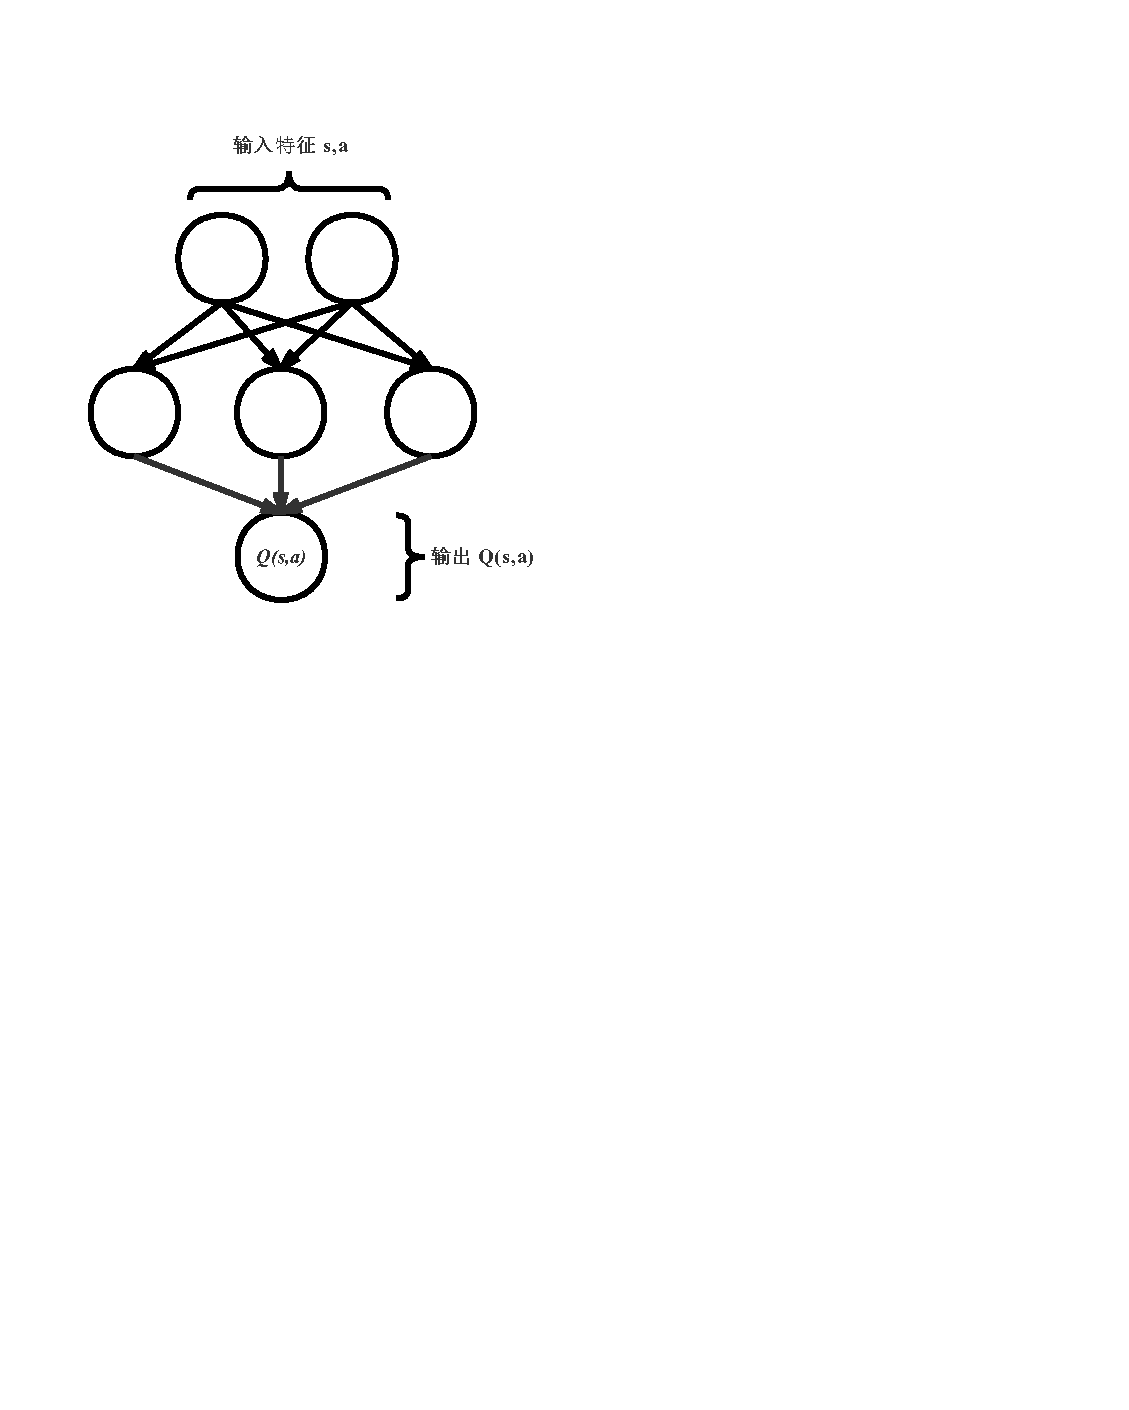
\includegraphics[width=0.5\textwidth]{DQN-show.pdf}
    \caption{Deep Q-Network 示意图}
\end{figure}

如上图所示,将实时数据流中的状态和行动作为特征向量传入神经网络的输入层,基于参数化的 Q-Learning 公式

\begin{equation}
\begin{aligned} \boldsymbol{w}_{t+1} =&\boldsymbol{w}_{t}-\alpha\nabla J(\boldsymbol{w}) \\ =&\boldsymbol{w}_{t}+\alpha\left[R_{t+1} - \gamma \max _{a} \widehat{Q}\left(S_{t+1}, a, \boldsymbol{w}_{t}\right)-\widehat{Q}\left(S_{t}, A_{t}, \boldsymbol{w}_{t}\right)\right]\\&\times\left[\gamma\nabla \max _{a} \widehat{Q}\left(S_{t+1}, a, \boldsymbol{w}_{t}\right)-\nabla \widehat{Q}\left(S_{t}, A_{t}, \boldsymbol{w}_{t}\right)\right] \end{aligned}
\end{equation}

通过神经网络的反向梯度传递来更新权值参数,进而实现梯度下降算法\cite{hecht1992theory}。称使用深度神经网络进行梯度下降的 Q-Learning 算法为 Deep Q-Learning 算法,将该神经网络结构称为 Deep Q-Network 。

在实际的应用场景中,不完全信息博弈常为多人对战类游戏,因此需要针对性地优化前面所描述的 Q-Learning 算法。

在 Q-Learning 中,基于 Bootstrap 思想,采用了 $\max_aQ(s,a)$ 作为 $Q(s,a)$ 的更新估计值,但在神经网络中大量使用 $\max$ 函数会带来一定的偏差值,带来决策误差。为了解决这一问题,需要使用两个神经网络交替使用来抵消这一偏差值。

\begin{Theorem}\label{the:doubledqn}
    记两个独立的 Deep Q-Network 分别为 $Q_1,Q_2$ ,并假定他们能无偏估计真实值,即满足条件 $\mathbb{E}\left[Q_1(s,a)\right] = q(s,a)$,$\mathbb{E}\left[Q_2(s,a)\right] = q(s,a)$ 。若使用 $Q_1$ 来参与行为决策,使用 $Q_2$ 来为相应的行为进行评估,最终所得到的评价值则为真实值的无偏估计。
\end{Theorem}

\begin{proof}
    由题设,$Q_1$ 用于行为决策,设 $A^*$ 为 $Q_1$ 决策出的最优策略,即有 $A^*=\mathop{\arg\max}\limits_aQ_1(a)$,此时 $A^*$ 的评价指标为
    \begin{equation}
        Q_2(S,\mathop{\arg\max}\limits_aQ_1(a)) = Q_2(S,A^*)
    \end{equation}
    根据题设条件
    \begin{equation}
        \mathbb{E}\left[Q_2(s,a)\right] = q(s,a)
    \end{equation}
    以及 $Q_1$ 与 $Q_2$ 互相独立,可知
    \begin{equation}
        \mathbb{E}\left[Q_2(S,\mathop{\arg\max}\limits_aQ_1(a))\right]=\mathbb{E}\left[Q_2(s,A^*)\right]=q(s,A^*)
    \end{equation}
    故行动 $A^*$ 的评价值 $\mathbb{E}\left[Q_2(s,A^*)\right]$ 是无偏估计值,证毕。
\end{proof}

因此根据定理 \ref{the:doubledqn} ,可以通过构建两个神经网络交替使用来抵消偏差值,使评估指标为真实值的无偏估计,从而可以确保在该评估体系下能够训练和学习出恰当的博弈策略。

在不完全信息博弈的实际应用场景中,会有 $N$ 名不同风格的选手对战,为了加强算法的自适应性和鲁棒性,需要进一步将 Deep Q-Network 模型分离为 $2N$ 个不同的神经网络,通过共同学习来消除因不同对手风格差异带来的影响,如下图所示。

\begin{figure}[H]
    \centering
    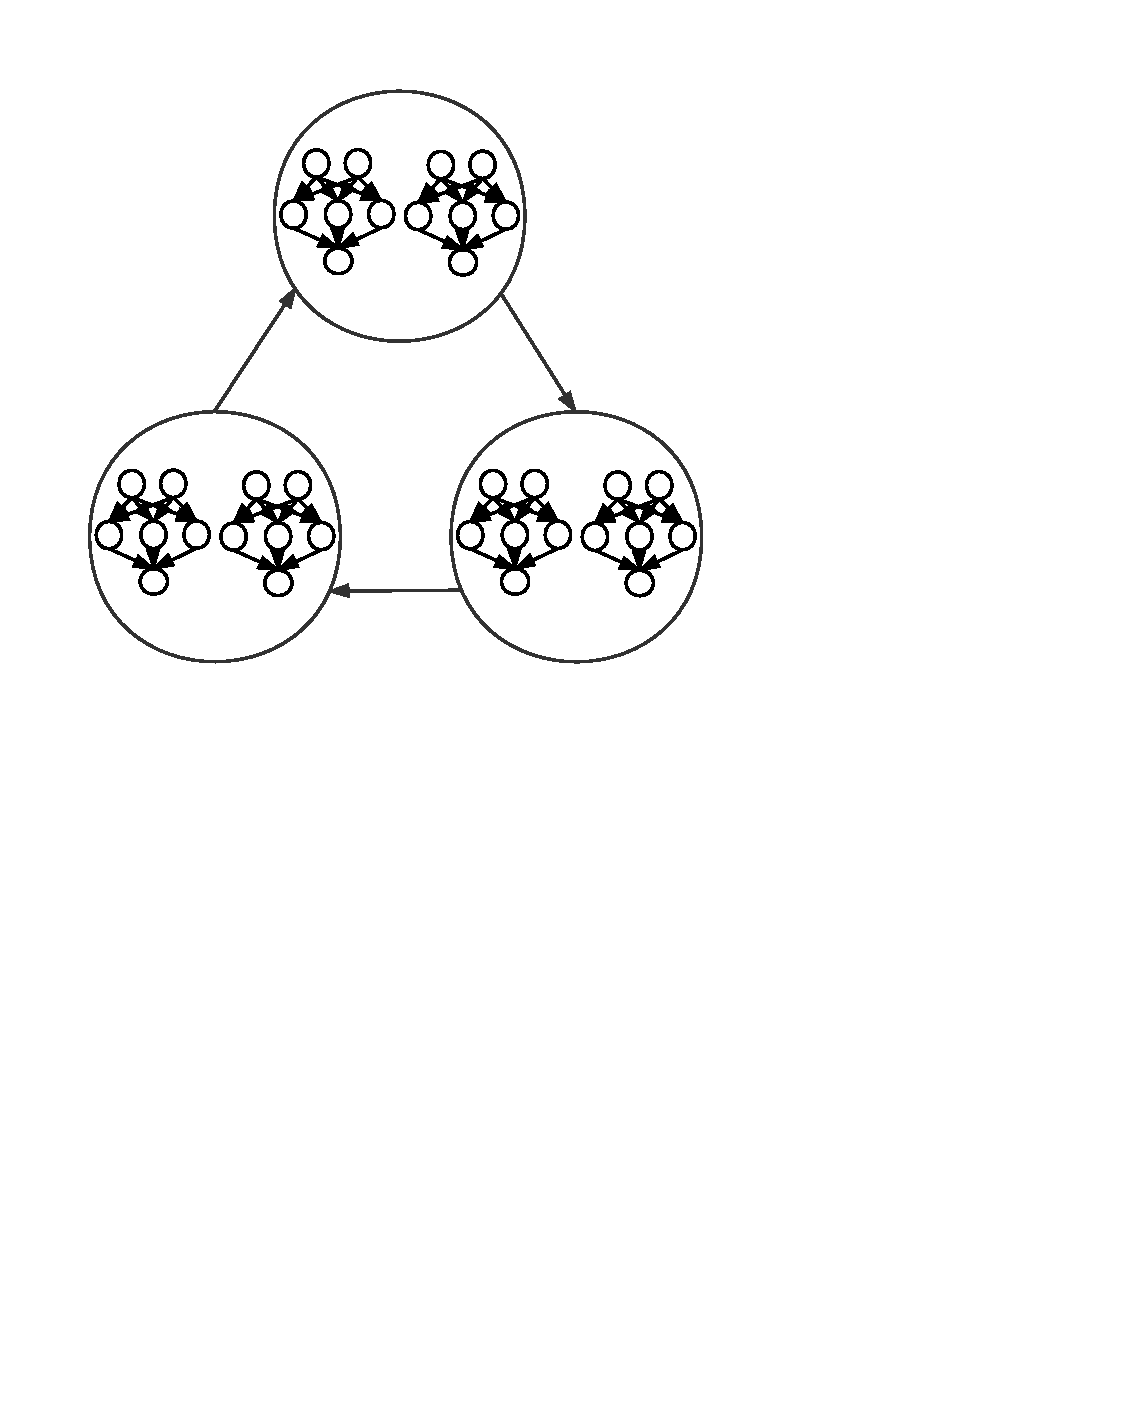
\includegraphics[width=0.6\textwidth]{Multi-DQN.pdf}
    \caption{自适应 Deep Q-Network (N=3)}
\end{figure}

如上图所示(图中 $N=3$),通过为每位选手分配一对 Deep Q-Network 之后,依次进行模拟博弈训练,基于训练数据执行 Deep Q-Learning 算法,通过前面的证明可知,这样的算法能够收敛得到 $Q(s,a)$ 函数的无偏估计值,便可基于估计函数 $\widehat{Q}(s,a)$ 推出最优策略 $\pi$ 。由于算法能够自适应地根据玩家数量调整网络参数,且每个玩家学习模型下的双神经网络能够自适应地准确消除各自的偏差,故称这样的算法为{\jiacu 自适应 Deep Q-Learning 算法}。
% !TeX root = ../main.tex
% -*- coding: utf-8 -*-

\chapter{仿真实验与评估}

我们选择一种简单的民间纸牌游戏,来验证前面所提出的强化学习理论是否能够较为适应地处理现实中的实际问题。

\section{实验环境建立}

\subsection{纸牌游戏的背景与规则介绍}

在本游戏中,初始牌面会去掉 “红桃2”、“梅花2”、“方块2”、“黑桃A”这 4 张牌,共计 48 张牌,每人发牌 16 张。第一回合由持手牌“黑桃3”的玩家出牌,随后依逆时针顺序跟牌,且要求在能出牌的情况下必须出牌,不可直接过牌。

作为第一位玩家出牌时,可任意选择牌型出牌,而跟牌阶段则只能按规则在指定牌型下出牌。该游戏规则简单,共有以下几种牌型:

\begin{center}
    \tablecaption{牌型介绍}
\begin{tabular}{|c|c|c|c|}
    \hline
    牌型简称 & 牌型描述 & 牌型简称 & 牌型描述 \\
    \hline
    对子 & 两张相同的牌 & 三条 & 三张相同的牌 \\
    \hline
    炸弹 & 四张相同牌 & 三带一 & 三条+单牌 \\
    \hline
    三带二 & 三条+任意两张牌 & 单顺 & 至少5张的连续牌 \\
    \hline
    双顺 & 至少2组连续对子 & 三顺 & 至少2组连续三条 \\
    \hline
    飞机 & 至少2组连续三带二 & 四带二 & 炸弹+任意两张牌\\
    \hline
\end{tabular}

\end{center}

最先将手牌出完的玩家为胜者。

\subsection{模拟建立的纸牌游戏环境}

基于游戏的基本规则,使用 \texttt{Python} 编程语言构建了一个简单的游戏模拟环境。为了能够进行数值化的模型训练,需要将不同纸牌转化为对应的数值编号,具体地,将游戏规则下一副牌(该规则下共 48 张牌)从 “黑桃3” 到 “方块2” 由小到大对应为一个长度为 48 的一维向量,每张牌都有一个唯一的 ID ,例如 \texttt{['黑桃3', '黑桃5', '红桃5', '梅花5', '黑桃7']} 转化后应为 \texttt{[0, 8, 9, 10, 16]}。后面的实验介绍中,模型内部结构均基于此前提。

在 \texttt{utils.py} 文件中,定义了 \texttt{divide\_cards()} 函数来实现发牌功能,能够随机将 48 张牌分为三份,发放给三位玩家,每位玩家各自分配到长度为 16 的一维向量,代表自己的手牌。

同时还定义了 \texttt{calculate\_score()} 函数,它能够根据游戏规则来计分,起到向模型传递反馈奖励值的作用。

在 \texttt{RunFastGame.py} 中,定义了一个完整的 \texttt{RunFastGameEnv} 类,它能够完整地模拟卡牌游戏对局,其中 \texttt{RunFastGameEnv.get\_state()} 函数能够获得当前所处的状态,\texttt{RunFastGameEnv.play\_cards()} 能够接收策略传入的指令来采取相应的行动。

具体地,\texttt{RunFastGameEnv} 能够模拟卡牌游戏对局中的每位玩家,它能基于环境信息以及模型的策略决策情况来模拟完整的游戏对局,从而产生了真实的经验数据,提供给模型进行 Monte Carlo 模拟,从而得以实现之前提出的算法。

\section{算法仿真与评估}

\subsection{Deep Q-Network 算法实现细节}

在 \texttt{DQN.py} 中,定义一个 \texttt{QNet} 类,建立一个全连接神经网络,其深度为 3 层。Input layer 有 209 个神经元,对应输入特征向量的 209 个元素;Hidden layer 1 有 512 个神经元;Hidden layer 2 有 256 个神经元;Hidden layer 3 有 128 个神经元;Output layer 只有一个神经元,其输出值为 $Q$ 函数所对应的值,如下图所示。

\begin{figure}[H]
    \centering
    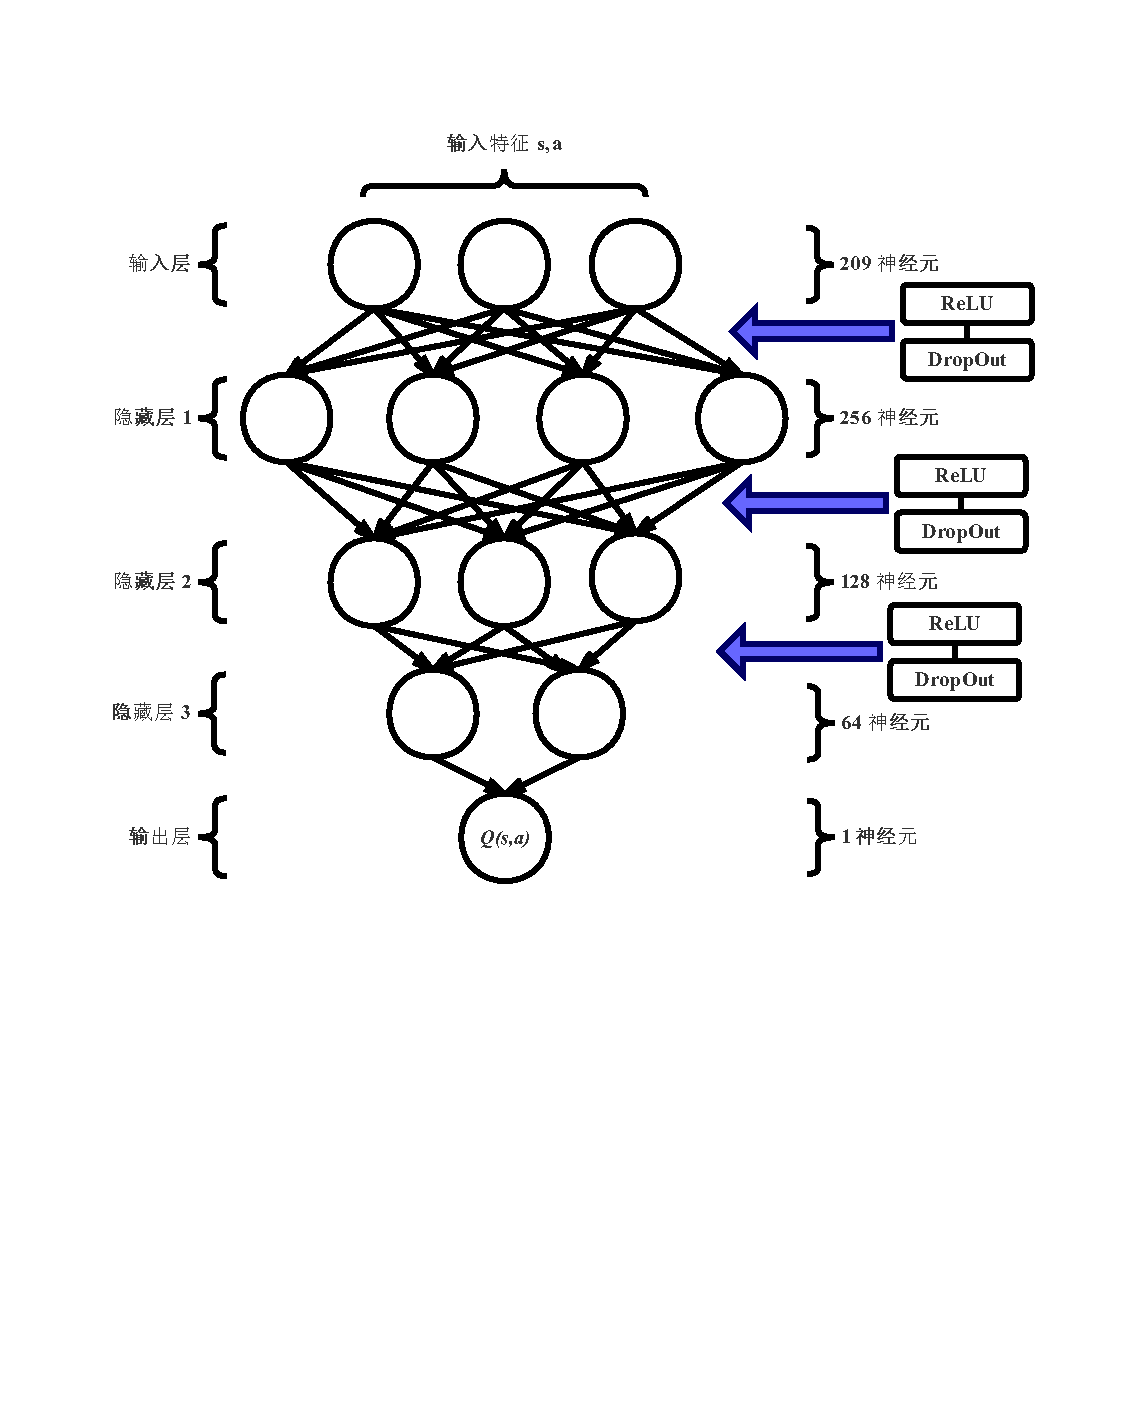
\includegraphics[width=\textwidth]{DQN-Detail.pdf}
    \caption{Deep Q-Network 实现细节}
\end{figure}

此外还定义了一个 \texttt{DQN} 类,用来实现 Deep Q-Network 的细节。其中,\texttt{DQN.choose\_action()} 函数代表策略函数 $\pi$ ,其功能是根据输入的状态 $s$ ,根据通过 $Q$ 函数大小决定的策略概率分布 $\pi(a|s)$ 来决定下一步应采取的行动 $a$ ;\texttt{DQN.store\_transition()} 函数和 \texttt{DQN.add\_reward()} 函数用于将模拟过程中的一些关键信息存储于记忆池中;\texttt{DQN.learn()} 函数的作用是将记忆池的信息提取出来,通过神经网络进行 Q-Learning 更新,更新公式为

\begin{equation}
    Q(S_t,A_t)\leftarrow Q(S_t,A_t)+\alpha\left[R_{t+1}+\gamma  \max\limits_aQ(S_{t+1},a)-Q(S_t,A_t)\right]
\end{equation}

最后,将 Deep Q-Network 模型接入进前面构建好的 \texttt{RunFastGameEnv} 环境下,即可开始模拟和训练的过程。

\subsection{仿真实验流程}

基于前面所描述的细节,本实验的具体流程如下:

\begin{algorithm}[H]
    \caption{训练过程}
    \begin{algorithmic}[1] %每行不显示行号
        \State 初始化三名不同的玩家 $A, B, C$
        \Repeat
        \State 开始新一局游戏,并为三名玩家发牌
        \Repeat
        \State 根据游戏规则决定当前回合应当出牌的玩家
        \State 进入当前玩家的视角,根据场面信息获取当前所处状态 $S$
        \State 将状态 $S$ 传入 $Q$ 函数 和 $\pi$ 策略,决策下一步所要采取的行动 $a$
        \State 实际采取行动 $a$ ,接收环境传递的反馈值,并存入记忆池
        \Until{执行行动 $a$ 后本局游戏分出胜负}
        \State 根据游戏规则,统计该局游戏各玩家得分,并追加存储至记忆池
        \State 将记忆池的信息,作为输入参数传入神经网络
        \State 经由神经网络完成一次训练学习,得到新的 $Q$ 函数和 $\pi$ 策略,用于下一次决策
        \Until{达到预设的训练次数}
        \State 结束训练,输出训练所得到的模型和参数
    \end{algorithmic}
\end{algorithm}

实验的流程图如下:

\begin{figure}[H]
    \centering
    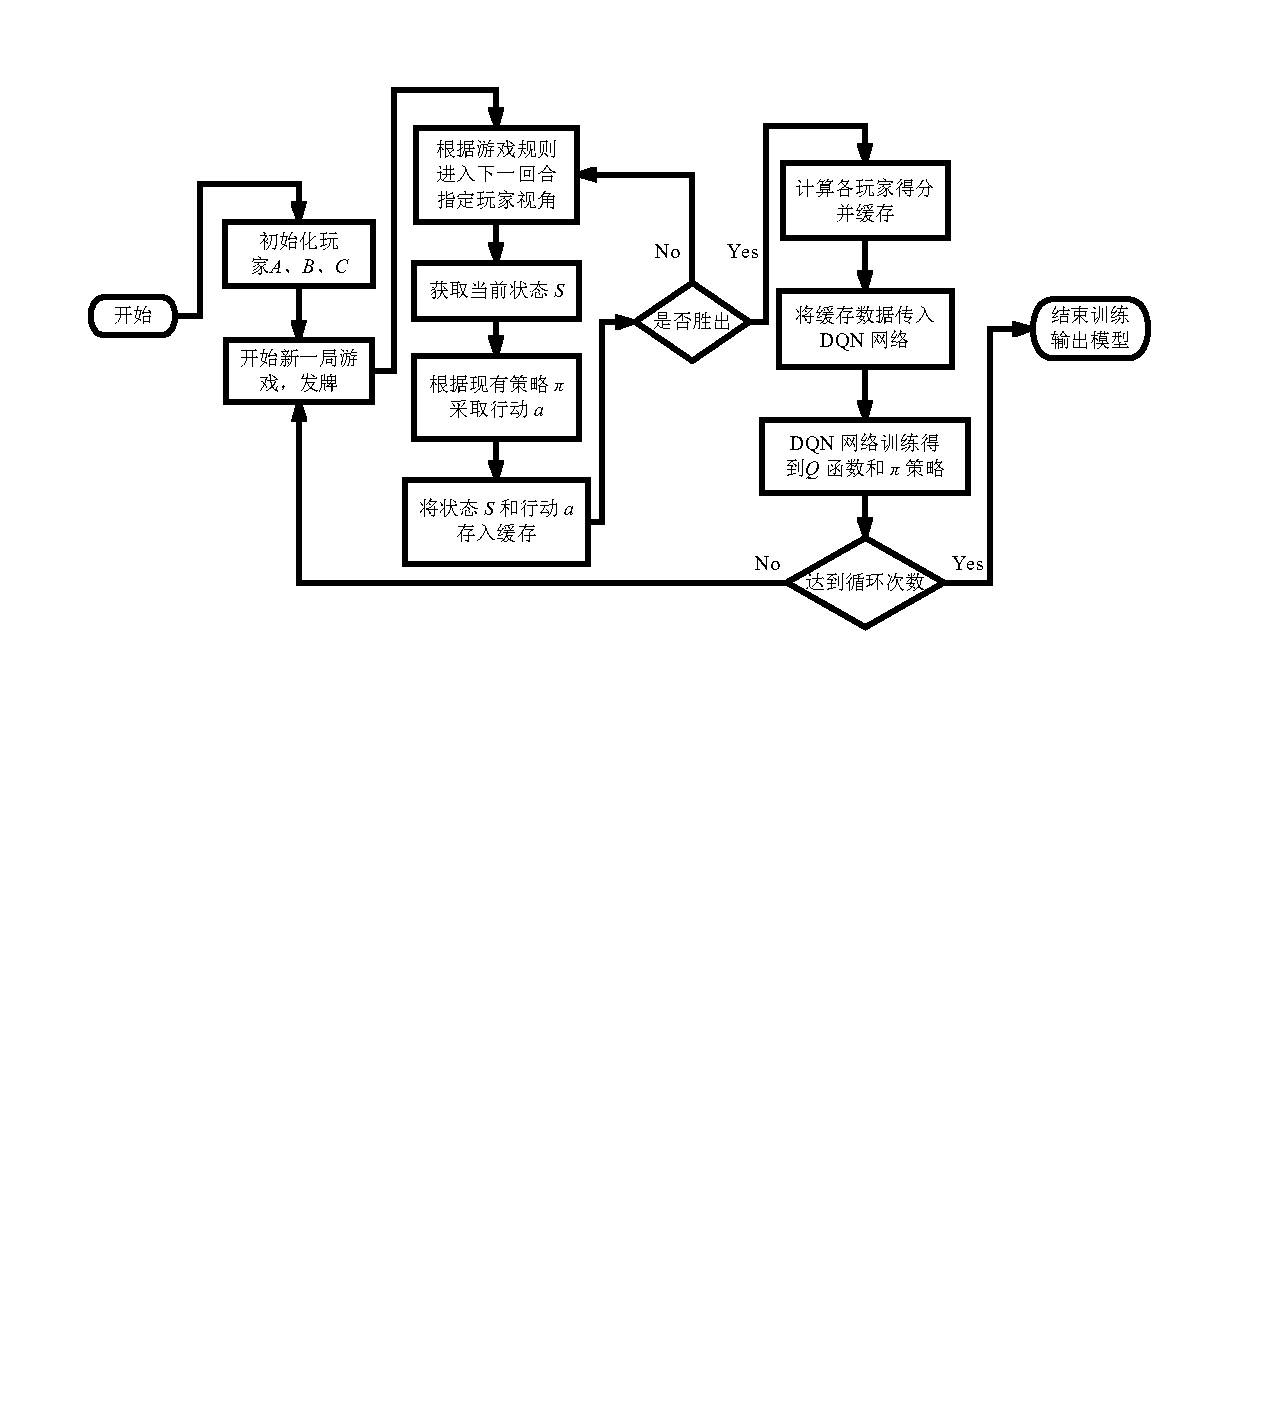
\includegraphics[width=\textwidth]{DQN-Process.pdf}
    \caption{实验流程图}
\end{figure}

\section{仿真实验结果与分析}

在自适应 Deep Q-Learning 算法中,

在 NVIDIA GTX 1080 GPU 的环境下,经过 50 万局自我对战学习(其中每 1000 局作为一个 epoch 集中学习),最终决策函数 $Q$ 得到收敛。

\begin{figure}[H]
    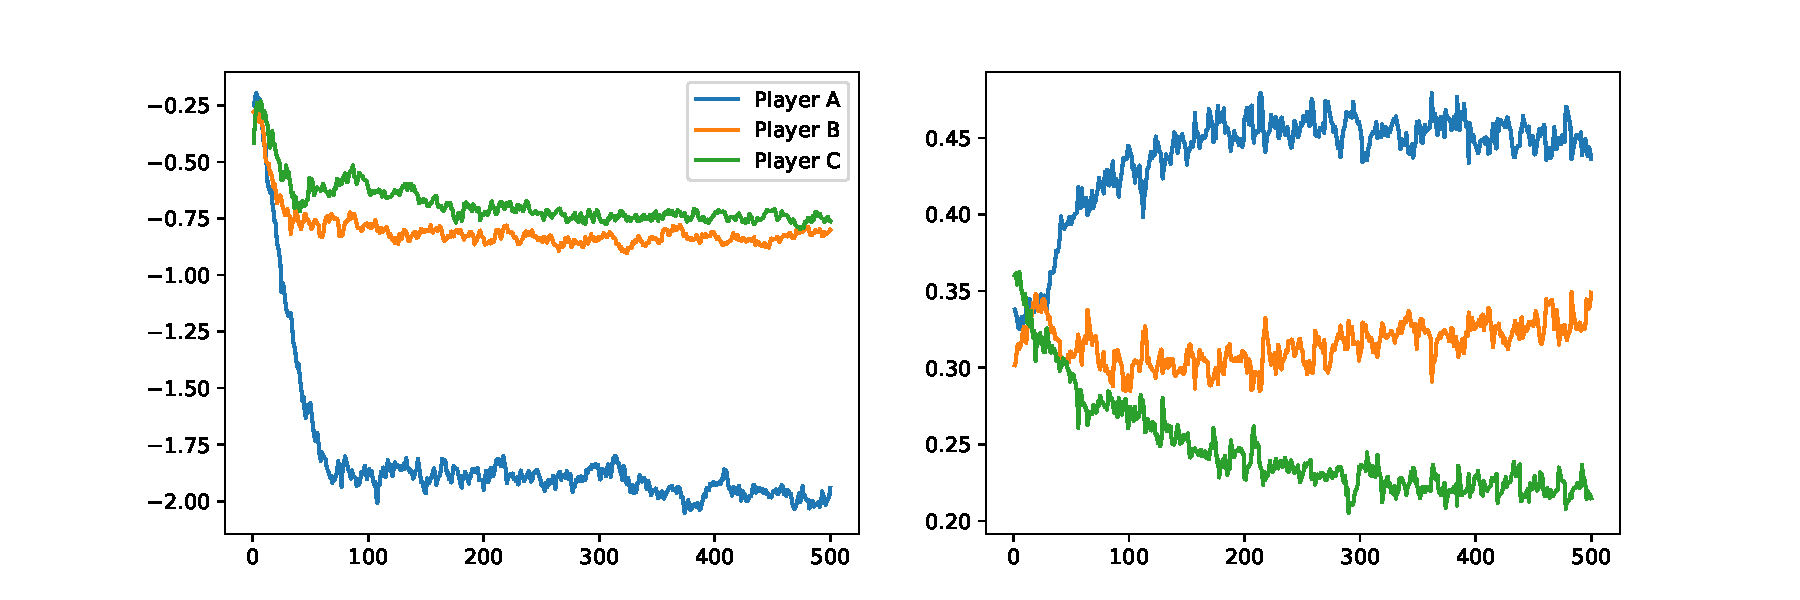
\includegraphics[width=\textwidth]{q-wr.pdf}
    \caption{Q 函数与实时训练胜率}\label{img:q-wr}
\end{figure}

从\ref{img:q-wr}的左图可以看出,经过自适应 Deep Q-Learning 算法训练可使行动价值函数 $Q(s,a)$ 收敛,进而可以得到 $\varepsilon$-贪心策略:

\begin{equation}
    \pi(a|s)=
    \begin{cases}
        \frac{\varepsilon}{|\mathcal A(s)|}&, a\neq\arg\max_aQ(s,a)\\
        1-\varepsilon-\frac{\varepsilon}{|\mathcal A(s)|}&, a=\arg\max_aQ(s,a)
    \end{cases}
\end{equation}

其中策略 $\pi(a|s)$ 是一个条件概率分布,其含义是模型处于状态 $s$ 时,决定采取行动 $a$ 的概率。

从\ref{img:q-wr}的右图可以观察发现,在训练过程中,最优算法模型的胜率不断上升并收敛,远优于另外两个普通的游戏模型,可以得知,自适应 Deep Q-Learning 算法确实通过强化学习的思想学习和掌握了一定的人类游戏技巧。


% !TeX root = ../main.tex
% -*- coding: utf-8 -*-

\chapter{总结与展望}

论文提出了能够解决多人博弈问题的“自适应 Deep Q-Learning 算法”。该方法将传统的理论强化学习方法与新兴的深度学习技术相结合,其创新点在于使用了双神经网络来抵消偏差,以及分离神经网络进行交互博弈,来进行自适应学习。

实验结果表明,该算法能够较好地解决不完全信息博弈问题,收敛速度快同时收敛效果好,且该算法短时间内能进行大量级的数据训练,算法效率高。但同时也还有着较大提升空间,有待进一步地加深研究。

随着机器学习理论的不断发展,其在实际中的应用也渐渐受到重视。传统的针对数据集内部关系问题的监督学习和无监督学习已经得到了广泛的研究,而新兴的实时反馈数据型博弈问题则渐渐成为一个关注的重点,这使得强化学习在机器学习中变得越发重要。

目前,对于简单的完全信息博弈问题,已经提出了许多有着不错成果的强化学习理论,如结合了 Monte Carlo 搜索树的 AlphaGo 算法\cite{silver2017mastering},但对于更实际且更复杂的不完全信息博弈问题,还尚未得到充分的研究,因此,针对不完全信息博弈问题的强化学习将会是未来的一个重要研究方向,有待进一步地充分研究。
% !TeX root = ../main.tex
% -*- coding: utf-8 -*-

\def\chapterformat{\bfseries\jiacu\zihaosi\heiti}
\printbibliography
\def\chapterformat{\centering\bfseries\jiacu\zihaosi\heiti}
% !TeX root = ../main.tex
% -*- coding: utf-8 -*-

%\makeschapterhead{致谢}
\chapter*{致谢}


% % !TeX root = ../main.tex
% -*- coding: utf-8 -*-


\end{document}
